\documentclass[twoside,twocolumn]{article}

\usepackage[utf8]{inputenc}
\usepackage{blindtext} 
\usepackage[sc]{mathpazo}
\usepackage[T1]{fontenc} 
\usepackage{times}
\usepackage{microtype} 
\usepackage[english]{babel} 
\usepackage[hmarginratio=1:1,top=32mm,columnsep=20pt]{geometry} 
\usepackage{booktabs} 
\usepackage{lettrine} 
\usepackage{enumitem} 
\setlist[itemize]{noitemsep} 
\usepackage{abstract} 
\renewcommand{\abstractnamefont}{\normalfont\bfseries} 
\renewcommand{\abstracttextfont}{\normalfont\small\itshape}
\usepackage{titlesec}
\renewcommand\thesection{\Roman{section}} 
\renewcommand\thesubsection{\roman{subsection}}

\titleformat{\section}[block]{\large\scshape\centering}{\thesection.}{1em}{}

\titleformat{\subsection}[block]{\large}{\thesubsection.}{1em}{} 

\usepackage{titling} 
\usepackage[hidelinks]{hyperref} 
\usepackage{graphicx}
\usepackage[export]{adjustbox}
\usepackage{caption}
\usepackage{pdfpages}
\usepackage{subcaption}
\usepackage{fancyhdr}
\usepackage{setspace}
\usepackage{mathptmx}
\usepackage{float}

\singlespacing
\setlength{\parindent}{0cm}
\setlength{\droptitle}{-4\baselineskip} 

\pretitle{\begin{center}\Huge\bfseries} 


\def\abstract
   {%
   \leftline{\normalsize \bf Abstract - }%
   \bf\small
   }

\def\endabstract
   {
   % additional empty line at the end of the abstract
   \vspace*{0.1in}% What about 1em instead?%
   }

\title{Experimento N°2\\El Osciloscopio} 
\author{
\textsc{William Guadalupe}\textsc{, Miguel Roca}\textsc{, Jesús Marin}\\
\normalsize Facultad de Ciencias \\ 
\normalsize Universidad Nacional de Ingenieria \\ 
\normalsize \href{mailto:wguadalupeq@uni.pe}{wguadalupeq@uni.pe},  \href{mailto:miguel.roca.a@uni.pe}{miguel.roca.a@uni.pe} \href{mailto:john@smith.com}{,  john3@smith.com} 
}
\date{\today}

\begin{document}

\maketitle

\begin{abstract}

En este experimento tomaremos medidas, usando
el sofware Multisim,analizando circuitos RC en serie y circuitos transitorios usando el osciloscopio con el fin de comprobar la constante de tiempo y el angulo de desfase y hallar los posibles errores de medicion.Se encontro que los errores de medicion se produjo en su mayoria al tomar los datos para el angulo de desfase usando el metodo de la elipse, esto es debido a que el osciloscopio no tiene demasiada presicion al querer hallar el a y b de la elipse.

\end{abstract}

\section{Introduccion}
El osciloscopio analogico y en particular el osciloscopio digital, es uno de los instrumento más útiles a la hora de querer representar cantidades como el voltaje o la intensidad de corriente versus el tiempo. No solo eso, su utilidad se extiende a la vida diaria en situaciones como: el valor de presión, el ritmo cardiaco, potencia de sonido, etc.\\
En este experimento, conoceremos los diferentes circuitos que se pueden armar y sus cantidades medidas por un osciloscopio.

\section{Objetivos generales y especificos}
\begin{itemize}
\item Familiariarze con el uso del osciloscopio digital en circuitos RC y de corriente alterna.
\item Hallar las mediciones de voltaje, frecuencia y desfasaje en los pasos apropiados.
\item Comparar los resultados teóricos (por ejemplo, el angulo de desfasaje hallado) con el experimental, y calcular los errores, de encontrarse.
\end{itemize}
\newpage
\section{Datos tabulados}
\begin{itemize}
\item Paso 1: Modelo y ancho de banda del osciloscopio y del generador.
\newline

\textbf{a)Osciloscopio}
\begin{table}[h]
\centering
\scalebox{1}{
 \begin{tabular}{|c|c|} \hline
    Marca y modelo & Tektronix TDS-2024 \\ \hline
    Ancho de banda & 200 MHz \\ \hline
  \end{tabular}
 }
\end{table}

    \textbf{b)Generador}
    \begin{table}[h]
    \centering
    \scalebox{1}{
     \begin{tabular}{|c|c|} \hline
        Marca y modelo & Agilent 33120A \\ \hline
        Ancho de banda & 4 digitos \\ \hline
    \end{tabular}
    }
    \end{table}

    
  \item Paso 2: Calibrar el Osciloscopio.\\

    Se procedió a calibrar correctamente los dos canales en tiempos de 0.5ms y 2V en la seccion de VOLT/DIV.\\
    
    \textbf{Señal de calibración}
    \begin{table}[h]
    \centering
    \scalebox{0.8}{
     \begin{tabular}{|c|c|} \hline
        f & 0.5 Hz \\ \hline
        $V_{pp}$ & 2 V \\ \hline
    \end{tabular}
    }
    \end{table}
    
  \item Paso 3-4: Medir las frecuencia del generador, medir el voltaje eficaz de las señales senoidales y cuadradas\\
\newpage
     \textbf{Medida del periodo y del voltaje eficaz}
    \begin{table}[h]
    \centering
    \scalebox{0.8}{
     \begin{tabular}{|c|c|c|c|c|} \hline
        Frecuencia nominal & 100Hz & 1KHz & 10KHz & 1MHz \\ \hline
        Período medido & 10 ms & 1 ms & 100 us & 1 us \\ \hline
        Vrms (señal senoidal) & 1.77 V & 1.77 V & 1.77 V & 1.77 V \\ \hline
        Vrms (señal cuadrada) & 2.5 V & 2.5 V & 2.5 V & 2.5 V \\ \hline
    \end{tabular}
    }
    \caption{Medida del periodo y del voltaje eficaz para señales senoidales y cuadradas}
    \label{tab:tabla de resistencia}
    \end{table}
    
\vspace{1cm}   
    \textbf{Calculo del error relativo}
    \begin{table}[h]
    \centering
    \scalebox{0.9}{
     \begin{tabular}{|c|c|c|} \hline
        Valor experimental & Valor teorico & Error relativo \\ \hline
        1.77 V & 1.77 V & 0 \\ \hline
        2.5 V & 2.5 V & 0 \\ \hline
    \end{tabular}
    }
    \caption{Errores relativos del voltaje eficaz}
    \label{tab:tabla de resistencia}
    \end{table}
    
\vspace{0.5 cm} 
\item Paso 5. Circuito RC, carga y descarga del condensador.\\

    \textbf{Analisis del circuito transitorio con señal directa}
    \begin{table}[h]
    \centering
    \scalebox{0.9}{
     \begin{tabular}{|c|c|c|c|c|} \hline
        R & C & \tau calculado & \tau medido & \% error \\ \hline
        10 k\Omega & 100 nF & 1 ms & 1 ms & 0 \\ \hline
        25 k\Omega & 240 nF & 6 ms & 5.999 ms & 0.017\% \\ \hline
        20 k\Omega & 330 nF & 6.6 ms & 6.599 ms & 0.015\% \\ \hline
    \end{tabular}
    }
    \caption{Calculo de la constante de tiempo en un circuito transitorio de señal directa}
    \label{tab:tabla de resistencia}
    \end{table}

\newpage
    \textbf{Analisis del circuito transitorio con señal cuadrada}
    \begin{table}[h]
    \centering
    \scalebox{0.9}{
     \begin{tabular}{|c|c|c|c|c|} \hline
        R & C & \tau calculado & \tau medido & \% error \\ \hline
        1 k\Omega & 100 nF & 100 \mu s & 100 \mu s & 0 \\ \hline
        10 k\Omega & 25 nF & 250 \mu s & 250 \mu s & 0\\ \hline
        5 k\Omega & 20 nF & 1.1 ms & 1.1 ms & 0\\ \hline
    \end{tabular}
    }
    \caption{Calculo de la constante de tiempo en un circuito transitorio de señal cuadrada}
    \label{tab:tabla de resistencia}
    \end{table}
    
\vspace{0.5cm}  
  \item Paso 6. Medicion del ángulo de desfase.\\   
    
    \textbf{Medicion del angulo de desfase en el eje de tiempos del osciloscopio.}
    \begin{table}[h]
    \centering
    \scalebox{0.9}{
     \begin{tabular}{|c|c|c|c|c|c|} \hline
        C1 & f & \Phi  calculado & Vep & Vsp & \Phi \\ \hline
        200 nF & 300 Hz & 20.67º & 2.49 V & 2.33 V & 22.70 º \\ \hline
        330 nF & 300 Hz & 32.14º & 2.49 V & 2.11 V & 30.37 º \\ \hline
    \end{tabular}
    }
    \caption{Calculo del angulo de desfase por los tiempos del osciloscopio}
    \label{tab:tabla de resistencia}
    \end{table}\\
    
\vspace{0.5cm}     
    \textbf{Medicion del angulo de desfase por el metodo de la elipse}
    \begin{table}[h]
    \centering
    \scalebox{0.9}{
     \begin{tabular}{|c|c|c|c|c|c|} \hline
        C1 & f & a & b & \Phi & \% \bigtriangleup \Phi / \Phi \\ \hline
        200 nF & 300 Hz & 1.48 & 4.68 & 18.44 º & 18.76\% \\ \hline
        330 nF & 300 Hz & 2.29 & 4.28 & 32.38 º & 6.618\% \\ \hline
    \end{tabular}
    }
    \caption{Calculo del angulo de desfase por el metodo de la elipse}
    \label{tab:tabla de resistencia}
    \end{table}\\
            
 \end{itemize}    
\newpage
\section{Cálculos, gráficos y resultados}     
 \textbf{Simulación del paso 3-4:}
  \begin{figure}[h]
    \centering
    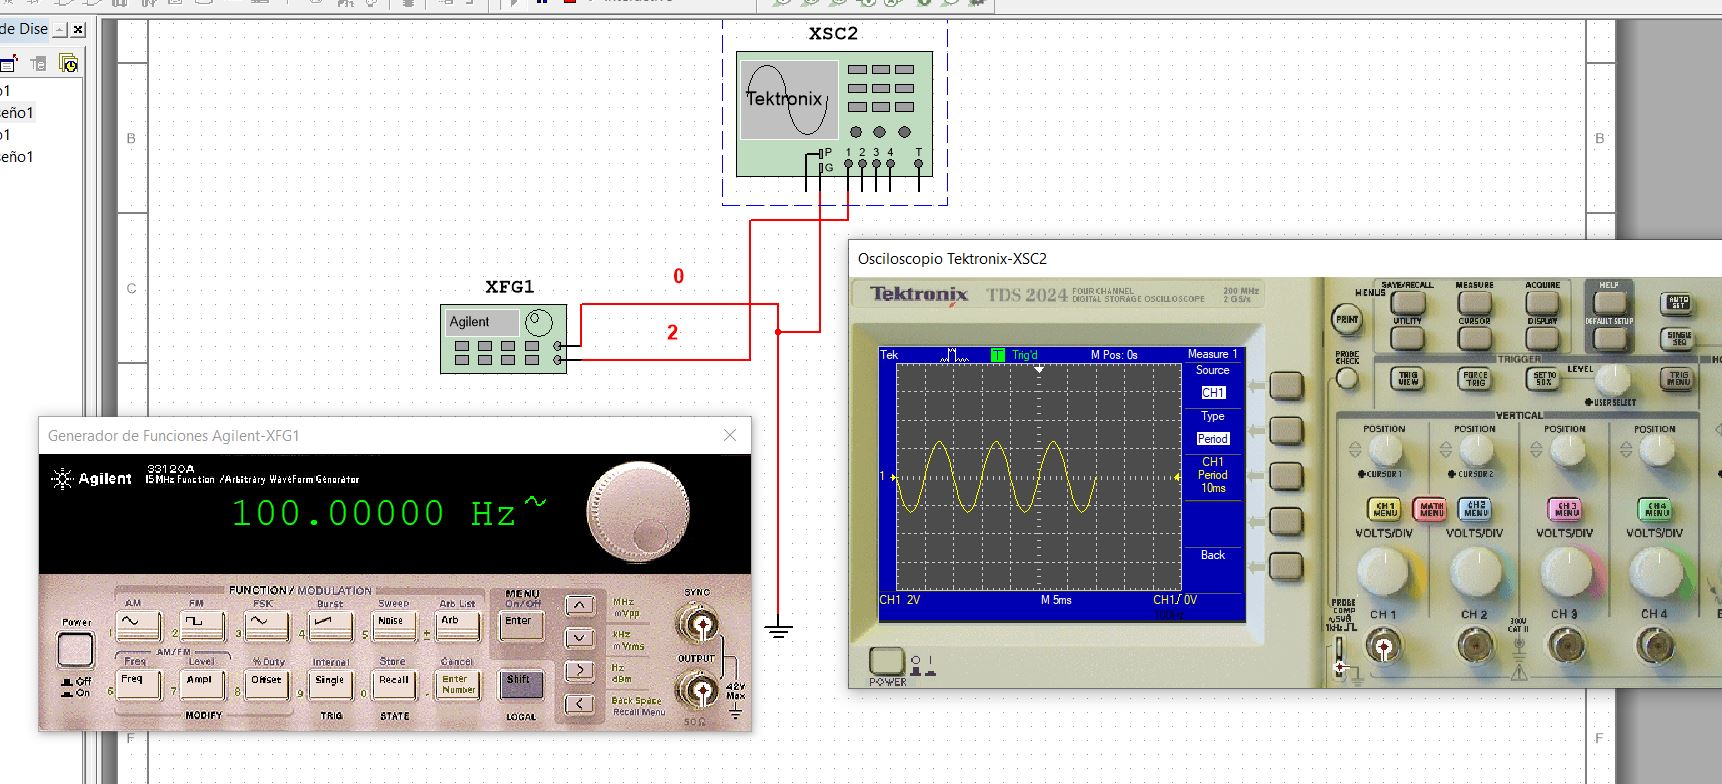
\includegraphics[scale=0.2]{Imagenes/2.1.JPG}
    \caption{Osciloscopio a una Frecuencia de 100Hz}
    \label{fig:circuito1}
  \end{figure}\\
  
  \begin{figure}[h]
    \centering
    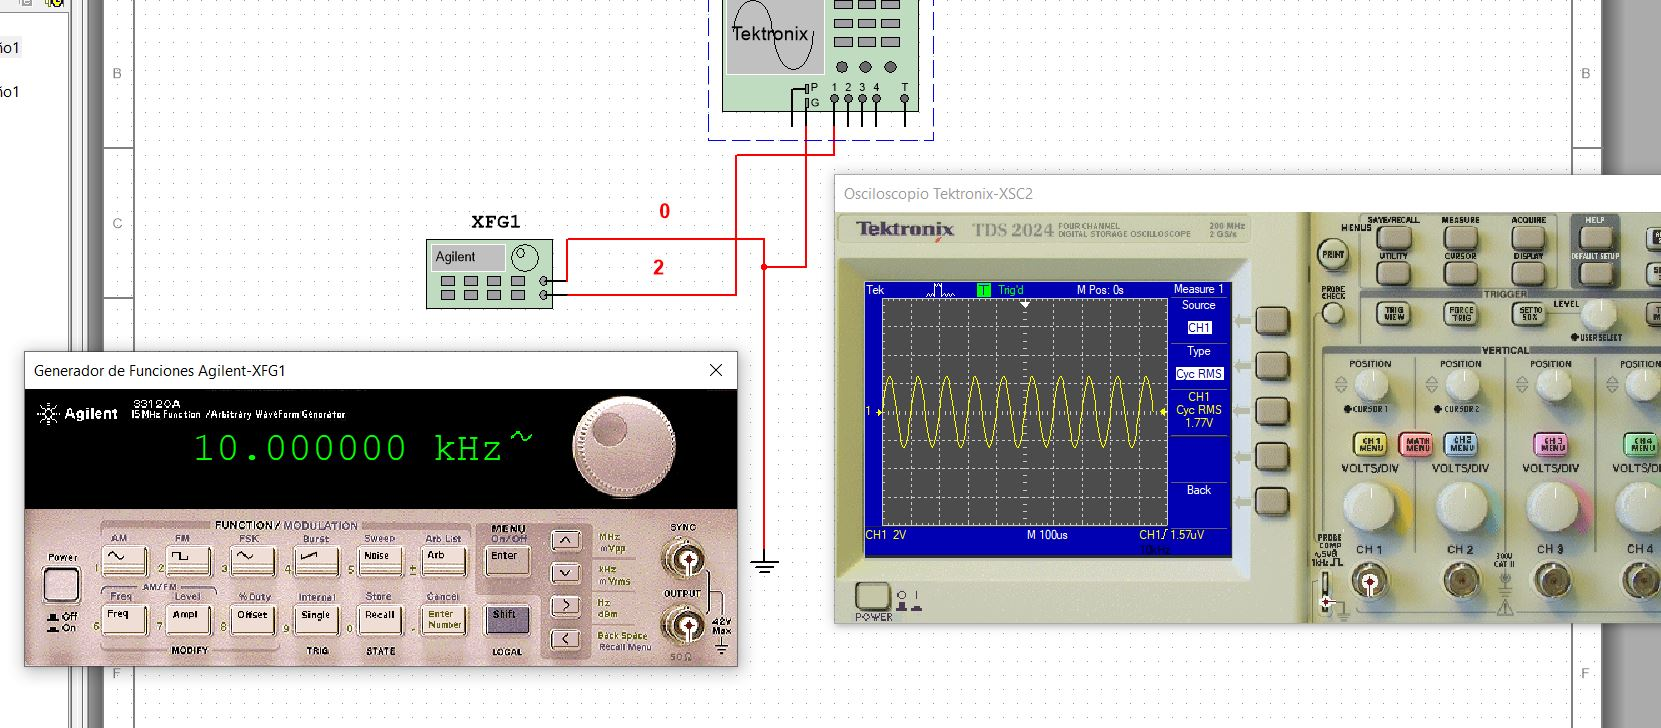
\includegraphics[scale=0.2]{Imagenes/2.2.JPG}
    \caption{Osciloscopio a una Frecuencia de 10kHz}
    \label{fig:circuito1}
  \end{figure}\\
\newpage  
 \textbf{Simulación del paso 5:}
  \begin{figure}[h]
    \centering
    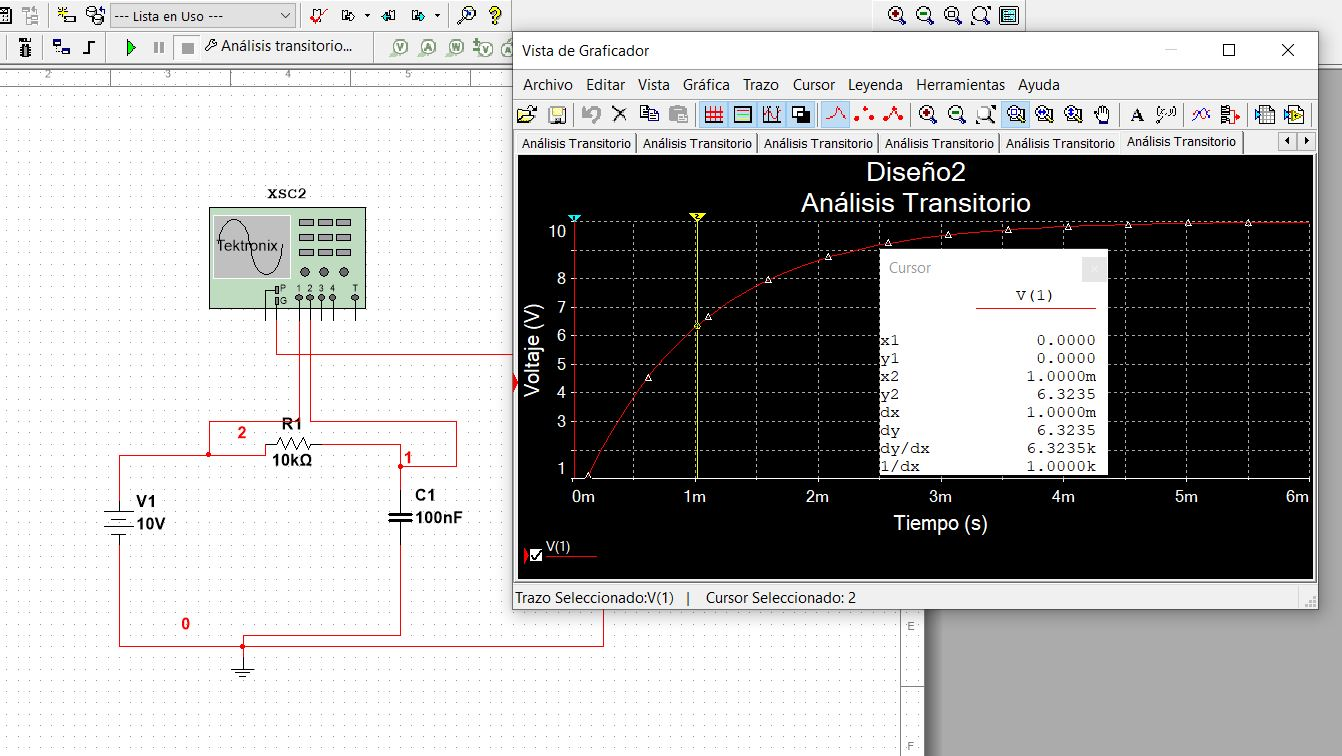
\includegraphics[scale=0.2]{Imagenes/3.1.JPG}
    \caption{Circuito Transitorio de señal directa para una R=10 kOhm y C=200 nF}
    \label{fig:circuito1}
  \end{figure}\\  

   \begin{figure}[h]
    \centering
    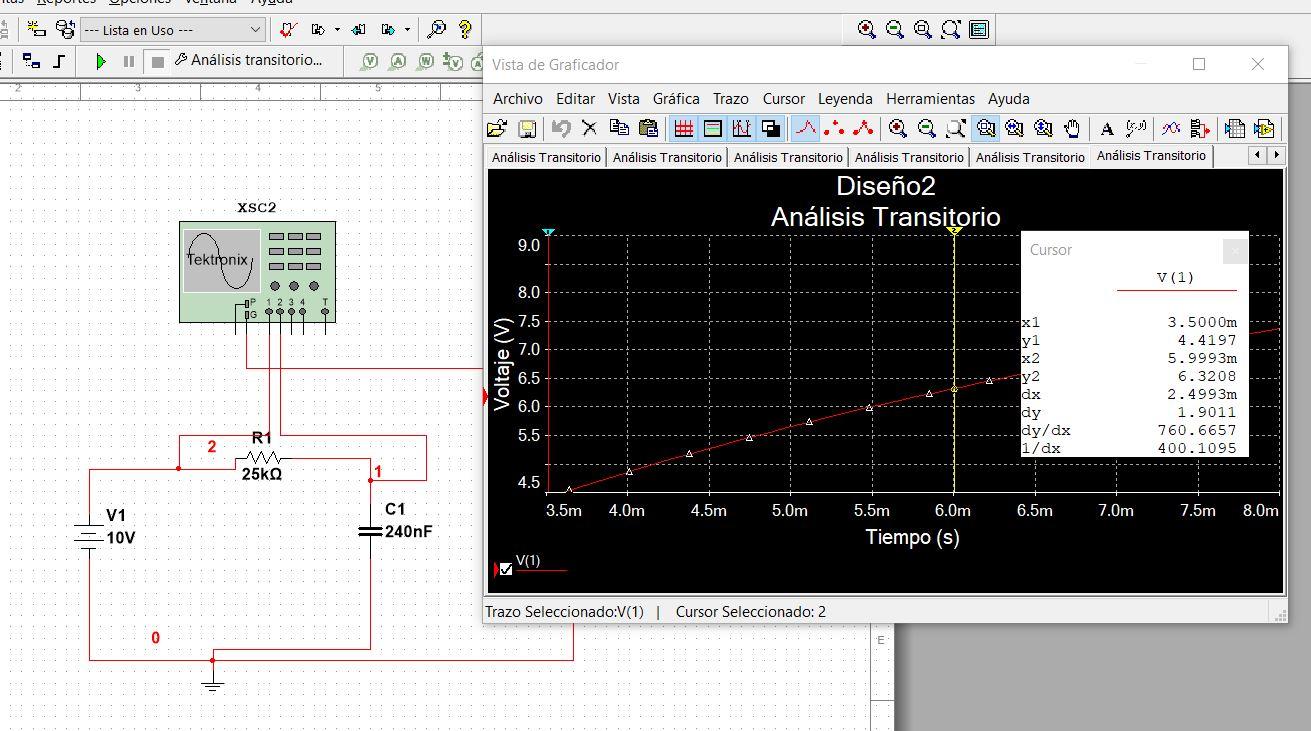
\includegraphics[scale=0.2]{Imagenes/3.2.JPG}
    \caption{Circuito Transitorio de señal directa para una R=25 kOhm y C=240 nF}
    \label{fig:circuito1}
  \end{figure}\\  
  
    \begin{figure}[h]
    \centering
    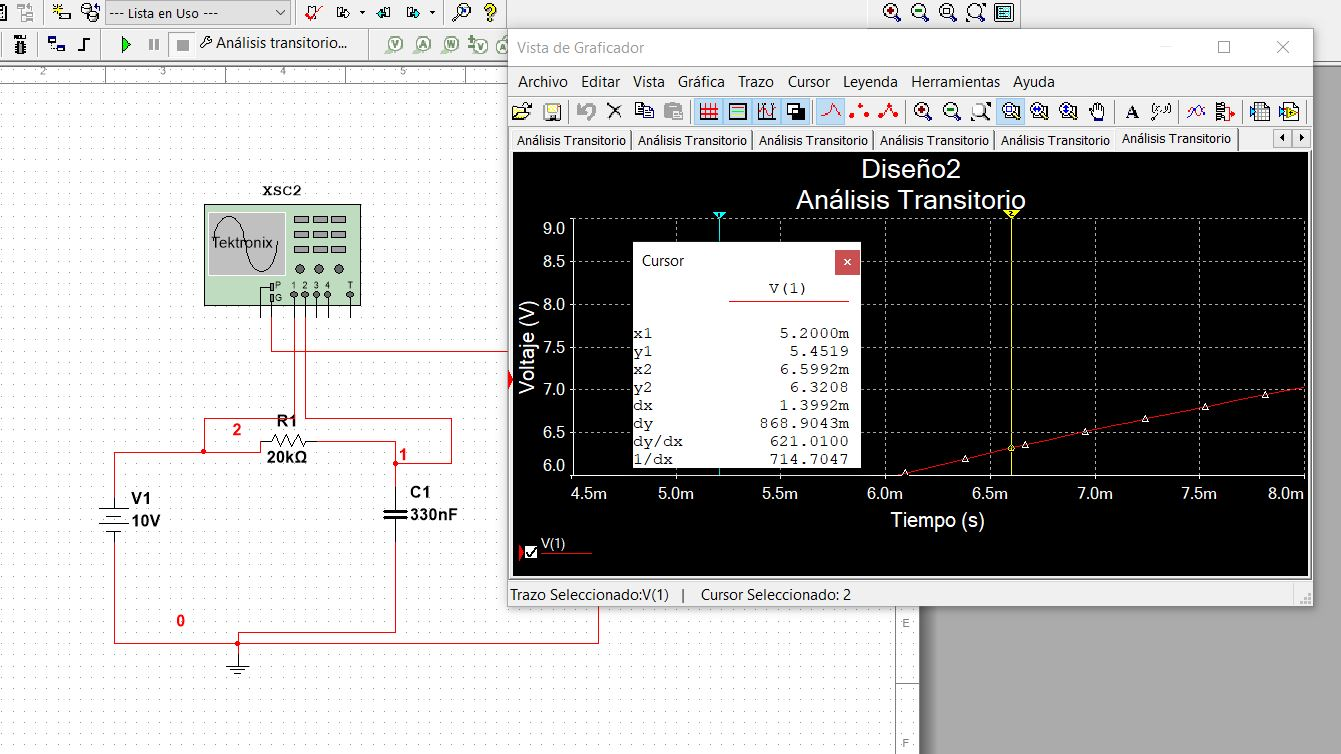
\includegraphics[scale=0.2]{Imagenes/3.3.JPG}
    \caption{Circuito Transitorio de señal directa para una R=20 kOhm y C=330 nF}
    \label{fig:circuito1}
  \end{figure}\\  

\newpage

    \begin{figure}[h]
    \centering
    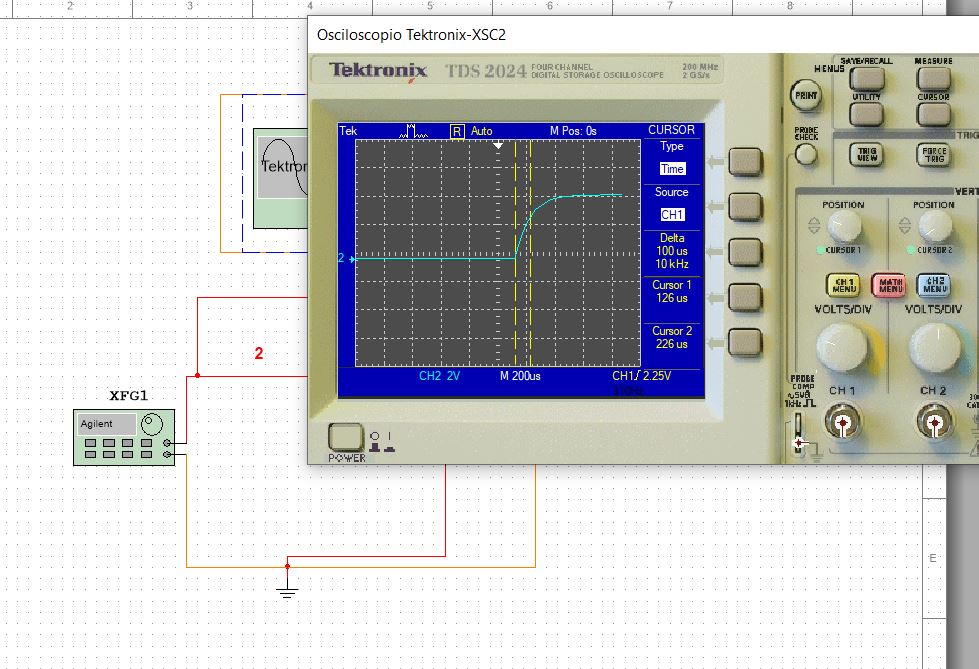
\includegraphics[scale=0.2]{Imagenes/4.1.JPG}
    \caption{Circuito Transitorio de señal cuadrada para una R=1 kOhm y C=100 nF}
    \label{fig:circuito1}
  \end{figure}\\  

    \begin{figure}[h]
    \centering
    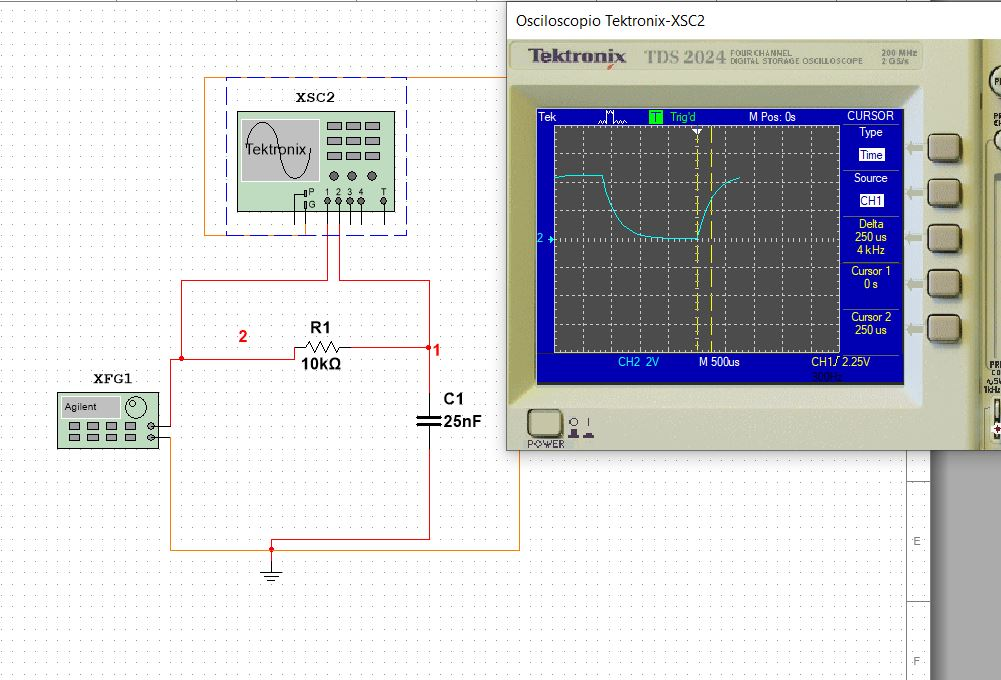
\includegraphics[scale=0.2]{Imagenes/4.2.JPG}
    \caption{Circuito Transitorio de señal cuadrada para una R=10 kOhm y C=25 nF}
    \label{fig:circuito1}
  \end{figure}\\    
  
    \begin{figure}[h]
    \centering
    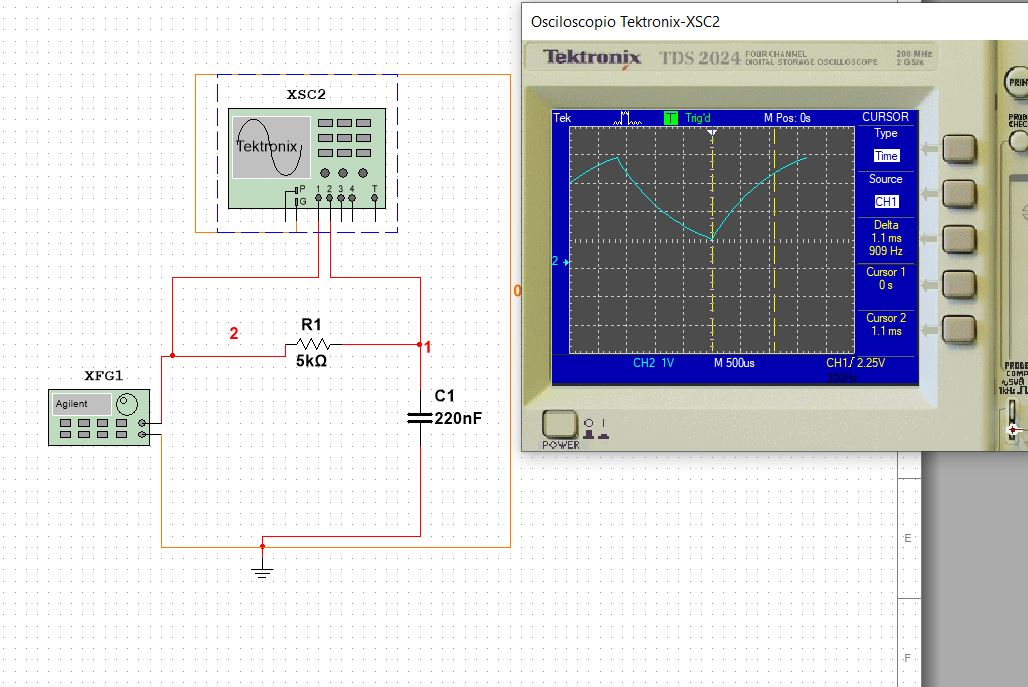
\includegraphics[scale=0.2]{Imagenes/4.3.JPG}
    \caption{Circuito Transitorio de señal cuadrada para una R=5 kOhm y C=220 nF}
    \label{fig:circuito1}
  \end{figure}\\   
\newpage
\textbf{Simulación del paso 6:}
  \begin{figure}[h]
    \centering
    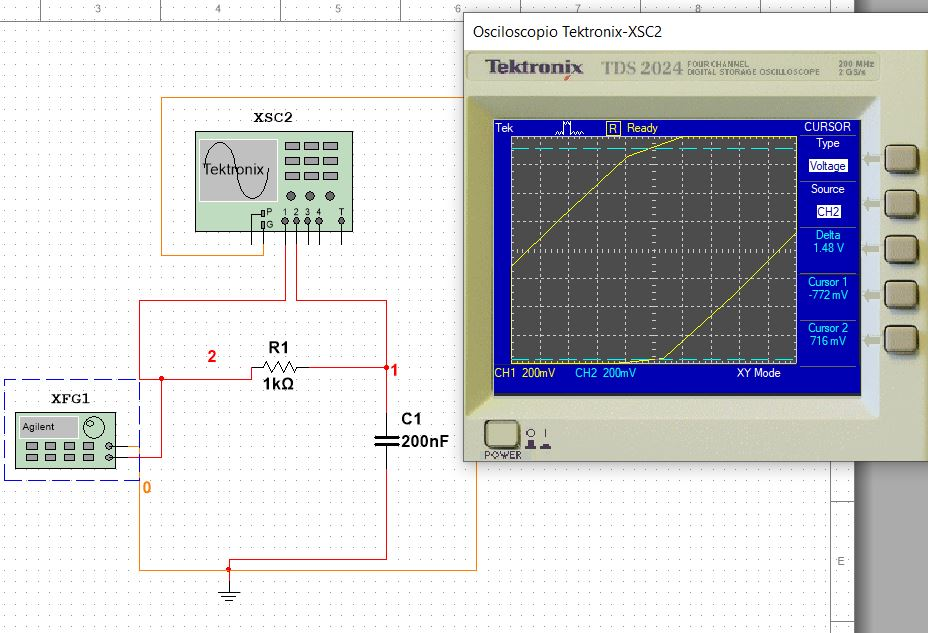
\includegraphics[scale=0.2]{Imagenes/5.3.JPG}
    \caption{Calculo del angulo de desfase (a) por metodo de la elipse para un C=200 nF y f=300 Hz}
    \label{fig:circuito1}
  \end{figure}\\  

    \begin{figure}[h]
    \centering
    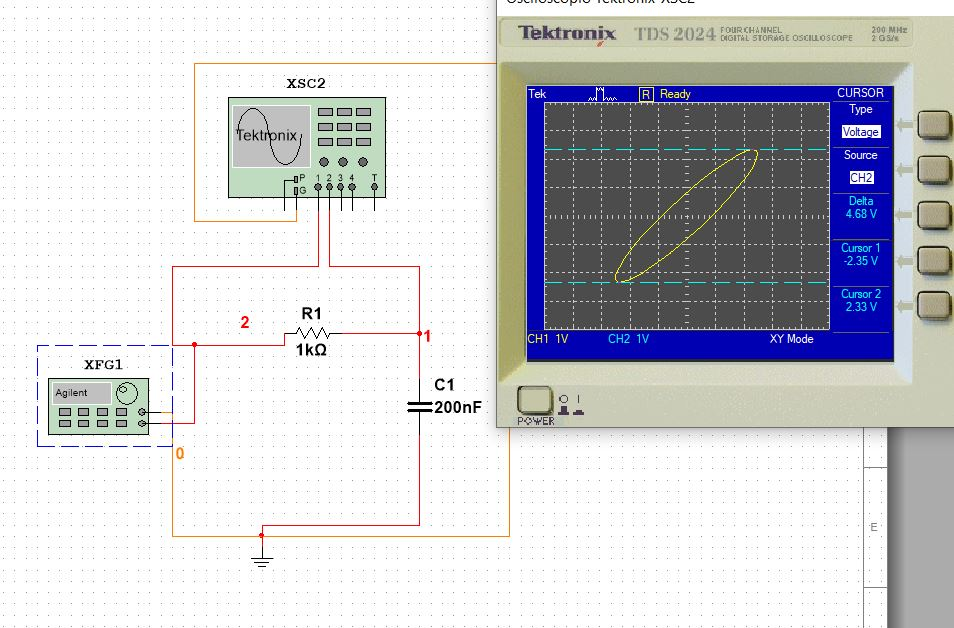
\includegraphics[scale=0.2]{Imagenes/5.4.JPG}
    \caption{Calculo del angulo de desfase (b) por metodo de la elipse para un C=200 nF y f=300 Hz}
    \label{fig:circuito1}
  \end{figure}\\  

  \begin{figure}[h]
    \centering
    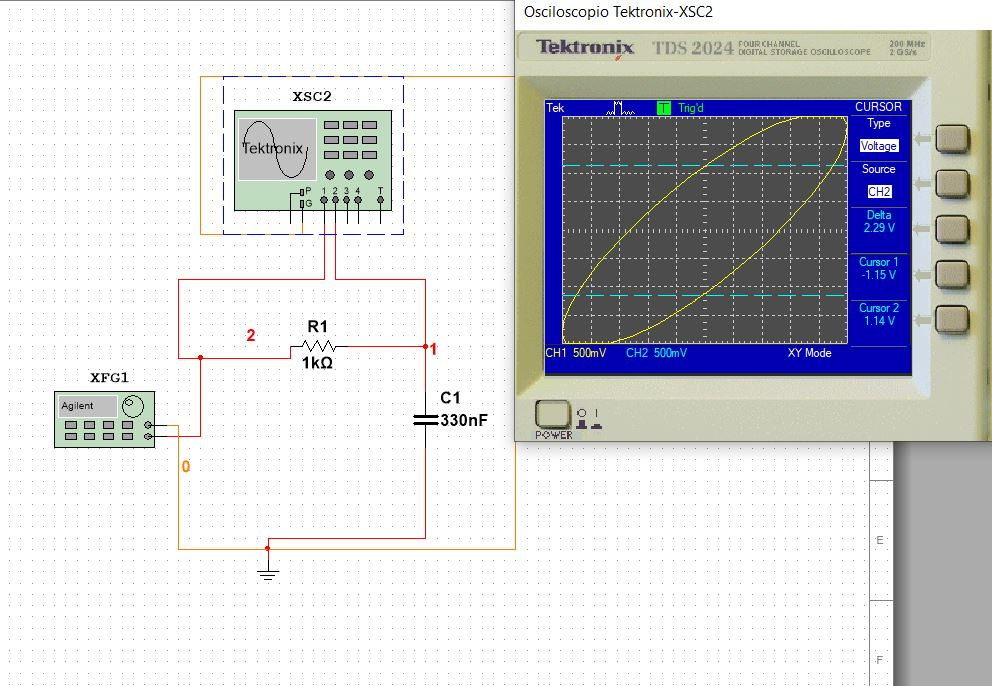
\includegraphics[scale=0.2]{Imagenes/5.5.JPG}
    \caption{Calculo del angulo de desfase (a) por metodo de la elipse para un C=330 nF y f=300 Hz}
    \label{fig:circuito1}
  \end{figure}\\  
  
\newpage
  
  \begin{figure}[h]
    \centering
    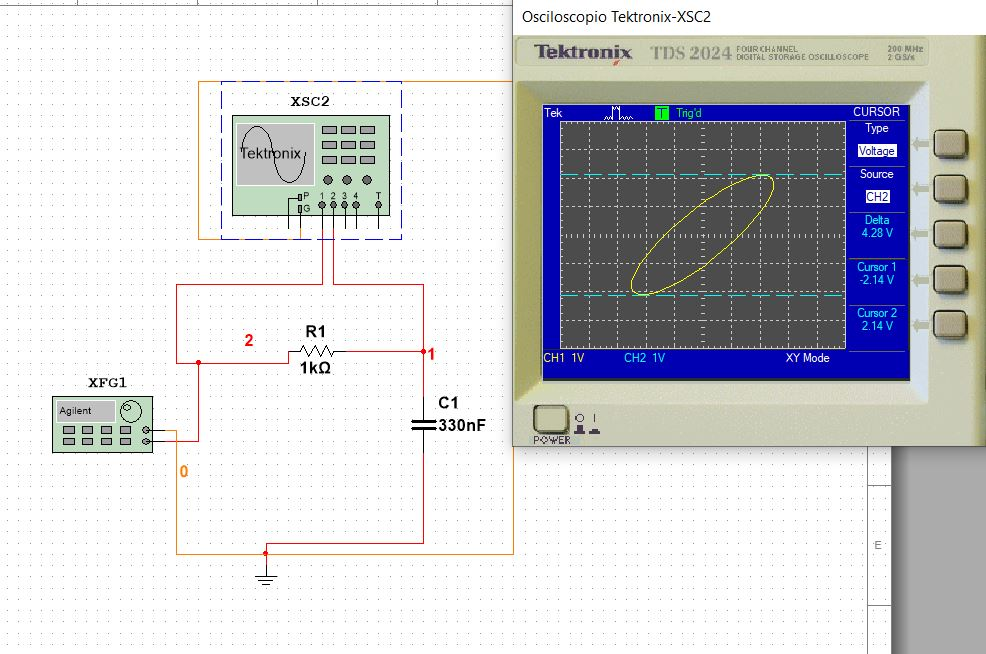
\includegraphics[scale=0.2]{Imagenes/5.6.JPG}
    \caption{Calculo del angulo de desfase (b) por metodo de la elipse para un C=330 nF y f=300 Hz}
    \label{fig:circuito1}
  \end{figure}\\  

\section{Discusión de los resultados} 

En general no hubo muchas complicaciones con el experimento ya que no se necesitaba de mucha presicion en el mismo, la unica excepcion a esa regla seria el paso 6 ya que el error relativo fue alto, sin embargo en los demas pasos no hubo error realtivo o fue muy bajo.

\section{Conclusiones}

\begin{itemize}

\item Comprobamos que la constante de tiempo en los circuitos transitorios solo depende de la resistencia del resistor y la capacitancia del capacitor

\item Comprobamos que el voltaje eficaz de la señal es igual al valor cuadratico medio de la señal

\item Denotamos la importancia de calibrar el osciloscopio ya que podriamos perder la señal del voltaje.

\item Aprendimos a como calcular el angulo de desfase ya sea por el metodo de la elipse o por los tiempos del oscloscopio

\end{itemize}

\section{Observaciones}

\begin{itemize}

\item El calculo del error relativo del angulo de desfase es, con diferencia, el paso con el error relativo mas grande, esto es debido totalmente a que a la hora de intentar hallar el lado a y b del elipse se comete muchos errores sistematicos ya que la presicion del osciloscopio virtual es muy limitado

\item En los demas pasos del experimento los errores relativos o son muy bajos o son nulos esto esdebido a que esas herramientas del laboratorio virtual empleadas en esos pasos son muy precisas y el error de medicion es casi nulo.

\end{itemize}

%	REFERENCE LIST
%----------------------------------------------------------------------------------------
\newpage
\begin{thebibliography}{99} % Bibliography - this is intentionally simple in this template

\bibitemCap 1 Guia para mediciones electrónicas.
Wolf – Smith, 1992, Prentice Hall
%\newblock Assortative pairing and life history strategy - a cross-cultural
%  study.
%\newblock {\em Human Nature}, 20:317--330.
 
\end{thebibliography}

%----------------------------------------------------------------------------------------


\end{document}
